Speech recognition is a complex technology which involves many fields, such as probability theory, machine learning, statistical natural language processing and speech processing. However, the architecture of a modern speech recognizer can be broadly divided into two main components namely the Acoustic Model (AM) and the Language Model (LM). The decoder uses these two components and produces the text output of the extracted input features as shown in Figure~\ref{fig:asr_component1}. 
\begin{figure}[ht]
\centering
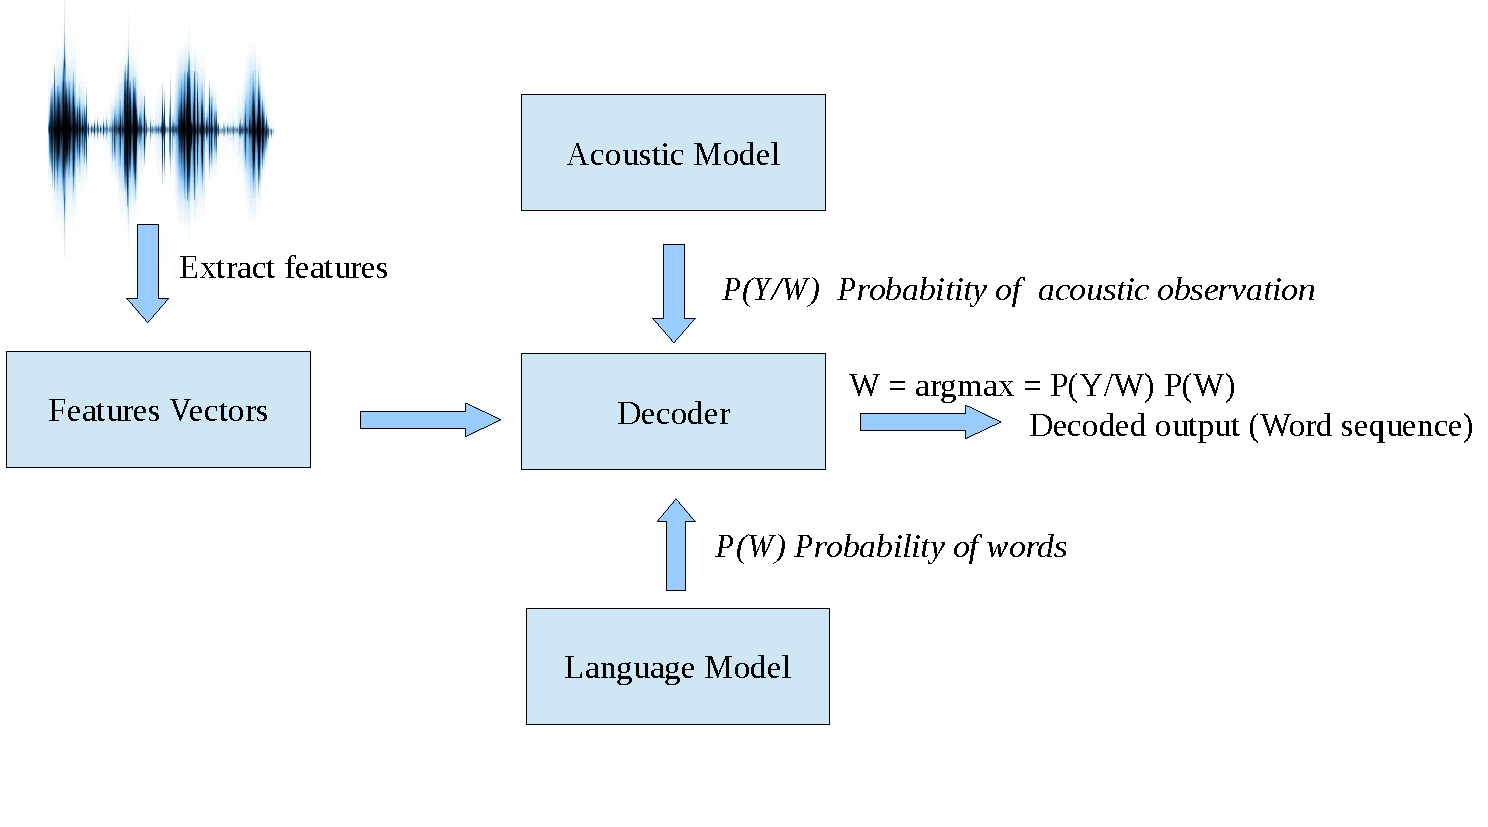
\includegraphics[width=\textwidth]{ASR_Component1.pdf}
\vspace{-1.2cm}
\caption{\textit{Basic components of speech recognition system.}}
\label{fig:asr_component1}
\end{figure}
If an utterance is represented as a sequence of words, $W$ = $w_1$, $w_2$, $w_3$, \dots \dots, $w_N$, then the decoder will try to find the most probable word sequence $\hat{W}$, given the sequence of acoustic vectors, $Y$ = $y_1$, $y_2$, \dots \dots, $y_T$. Using Byes rule, the probability of a word given an observation $P(W/Y)$ can be found as: 
\begin{equation}
\label{equ:bayes_rule}
\hat{W} = \argmax P(W/Y) = \argmax\frac{P(W)P(Y/W)}{P(Y)}.
\end{equation}
In this equation, the word sequence $\hat{W}$ must be found, as the one that maximizes the product of $P(W)$ and $P(Y/W)$, where $P(W)$ is the prior probability which comes from the language model and $P(Y/W)$ is the probability of vector sequence $Y$ given some word sequence $W$, which is known from the acoustic model. $P(Y)$ is ignored, as it is a constant for all possible word sequences. Below each of the component is explained in more detail.
\subsection{Acoustic modeling}
The performance of the speech recognition systems mostly depends on a good acoustic model. Acoustic modeling for speech recognition refers to the process of how one can statistically represent the features vectors sequences, which are computed from the continuous speech. Since, it is difficult to have frequent number of each word in the training data to accumulate acoustic statistics for that word, therefore, each word is represented into smaller units of speech called the phonemes. This is usually called the  "pronunciation modeling". In modern speech recognition systems, approximately 39-45 phonemes are used, which are combined to form all possible words in English. To model the acoustic features, Hidden Markov Model (HMM)~\cite{hmm_for_SR} are used. Acoustic modeling is explained in more details in the next chapter.

\subsection{Language modeling}
The language modeling (LM) specifies what sequence of words to expect in the speech given the previous word or sequence of $N$ words. In equation~\ref{equ:bayes_rule}, the term $P(W)$, represents the language model. Many techniques have been used to estimate the probability, $P(W)$. Two of the most important techniques are mentioned below.
\subsubsection{Formal language models} 
\label{sec:gramar_based_lm}
The formal or grammar based language model is composed of a grammar and a parsing algorithm. The grammar specifies allowable structure of a language and the parsing specifies the analysis method to check if rules of the grammar are respected. For small size recognition task, often the grammar based language model is a good solution. 
\subsubsection{Probabilistic language models}
\label{sec:prob_lang_model}
The probabilistic language models assigns probabilities to words $\textit{W}_k$ based on preceding words $\textit{W}_k^{k-1} = \textit{w}_1 , \cdots \cdot,\textit{w}_{k-1}$  from a training corpus. The most commonly used language model from this category are the $N$-gram language models, where $N$ means number of preceding words to be considered. Some variations are \textit{unigrams}, \textit{bigrams} and \textit{trigrams}. 

For \textit{trigrams}, where \textit{N=3} we can calculate the probablity as:
\begin{equation}
  \hat{P}(w_k | w_{k-1},w_{k-2}) = \frac{c(w_{k-2},w_{k-1},w_k)}{n(w_{k-2},w_{k-1})} 
\end{equation}
where $c(w_{k-2},w_{k-1},w_k)$, specifies the number of times, the words $w_{k-2},w_{k-1}$ and $w_k$ comes together and $n(w_{k-2},w_{k-1})$, specifies the number of times the words $(w_{k-2},w_{k-1})$ occurs together. 

For a vocabulary $V$ of 10,000 words, the \textit{trigrams} size equals to $V^3$, which is a large number and not all of the \textit{trigrams} appears in the training data. To avoid the training data sparsity problem for LM, some other techniques such as \textit{liner interpolation}, \textit{discounting techniques}~\cite{good1953population} and \textit{backing-off}~\cite{s_m_katze, ney94} LMs are used.

\subsubsection{Language model for elevator}
